\documentclass{beamer}
\usepackage[T1]{fontenc}
\usepackage[spanish]{babel}

\usetheme{hannover}

\title{Moogle}
\author{Salma Fonseca Curbelo}

\begin{document}

\begin{frame}   
\maketitle
\end{frame}

\begin{frame}
    
    \frametitle{Introducción} 

    En esta presentación se explicarán los pasos que se siguieron para desarrollar el primer proyecto de programación,
    cuyo objetivo es  implementar el motor de búsqueda de Moogle!,
    una aplicación cuyo propósito es buscar inteligentemente un texto en un 
    conjunto de documentos.
    
\end{frame}

\begin{frame}
    \frametitle{Cargar Documentos}

\begin{enumerate}
    \item Se ejecuta el método \textit{GetDocuments} de la clase \textit{Documents}.
    \begin{figure}[h]

        \centering
        \label{imag: obtdocs}
        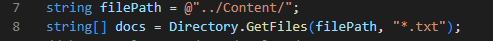
\includegraphics[width=11cm]{ObtenerDocs.png}
        \caption[]{\footnotesize Obtener direccion de documentos}

    \end{figure}

    \item Se lleva a cabo un ciclo foreach para obtener el texto de los documentos con la función \textit{ReadAllText}
    
    \begin{figure}[h]
        \centering
        \label{imag:cargardocs}
        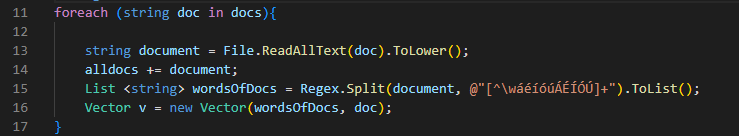
\includegraphics[width=10cm]{CargarDocs.png}
        \caption[]{\footnotesize Obtener contenido de documentos}
    \end{figure}

\end{enumerate}
    
\end{frame}

\begin{frame}
    \frametitle{Construcción de vectores}

    Cada vector representará un documento y tendrá como propiedades:

        \begin{itemize}
            \item  \textbf{Vectorwords:} se le asigna la lista de string que recibe como parámetro (cada palabra del documento).
            \item  \textbf{CantidadPalabras:} se le asigna el tamaño de la lista que se recibe.
            \item  \textbf{Path:} se le asigna el string que recibe como parámetro (dirección del documento).
        \end{itemize}

\end{frame}

\begin{frame}
    \frametitle{<Calculo TF, IDF>}

    \begin{itemize}
        \item El método \textit{GetDocuments} entrará en otro ciclo que, para cada vector de la lista \textit{files} en la clase \textit{Matrix}, 
        se llama al método \textit{CalculateTFIDF}

        \begin{figure}[h]

            \centering
            \label{imag: calculoTFIDF}
            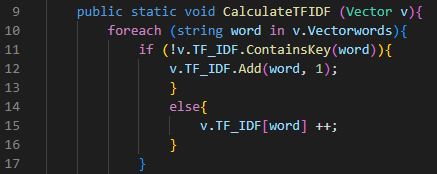
\includegraphics[width=9cm]{CalcularTFIDF.png}
            \caption[]{ \footnotesize Método para calcular repetición de palabras}
        
        \end{figure}

        \item foreach que recorrerá cada palabra que se encuentra en las claves del diccionario y asi obtener la cantidade
        de veces que está reoetida la palabra.

    \end{itemize}

\end{frame}

        \begin{frame}
            \frametitle{<Calculo TF, IDF>}

            \begin{itemize}
                \item Se calcula el TF
        
        \begin{figure}[h]

            \centering
            \label{imag: TF}
            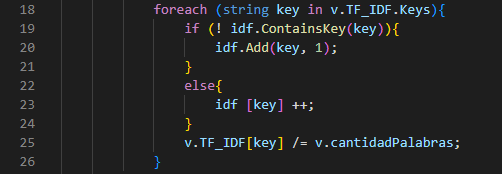
\includegraphics[width=9cm]{TF.png}
            \caption[]{ \footnotesize Método para calcular TF}
        
        \end{figure}

        \item Se calcula el IDF
        
        \begin{figure}[h]

            \centering
            \label{imag: IDF}
            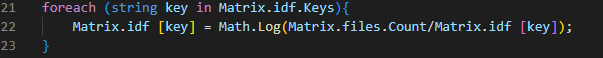
\includegraphics[width=13cm]{IDF.png}
            \caption[]{ \footnotesize Método para calcular IDF}
        
        \end{figure}

            \end{itemize}
        
        \end{frame}

        \begin{frame}
            \frametitle{<Búsqueda>}
        
            \begin{itemize}
                \item Se ejecuta la función \textit{Search} dentro de la clase \textit{Moogle},
                que recibirá como parámetro el query que se introdujo.
                \item Se convierte el query a una lista de string \textit{query} y llevándolo a una lista con la
                 función \textit{ToList}
                \item Se calcula el score
            \end{itemize}
        
        \end{frame}

        \begin{frame}
            \frametitle{Cálculo del score}

            Se realiza la siguiente operación:

\begin{equation}
    \centering
  \sum  tfidf \cdot  idf \cdot tf
\end{equation}

Refiriéndoe al tfidf de la palabra en el documento, al idf propio de la palabra y al tf de la palabra en el query. Para saber la cantidad de veces que se encuentra la palabra en el query se
utiliza la función \textit{Count}.
        
        \end{frame}

        \begin{frame}
            \frametitle{Resultado de la búsqueda}

            Solo se añade el documento a la lista de SearchItem, 
            llamada \textit{result} si el score es mayor  que 0 y se muestra:

        \begin{itemize}
            \item El score
            \item El nombre del documento con la función \textit{GetName} 
            \item El Snnipet, que se obtiene mediante la función \textit{Snippet}
            
            \begin{figure}[h!]

                \centering
                \label{imag: snippet}
                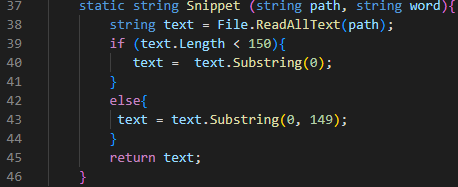
\includegraphics[width=9cm]{Snippet.png}
                \caption[]{ \footnotesize Método para crear el Snippet}
            
            \end{figure}
            
        \end{itemize}
        \end{frame}

\end{document}